
\chapter{Data imputation}
\label{ch:data-imputation}

\section{Model estimation}

Whenever some variables are measured, there is a chance of failing on collecting the data and missing some samples. It could be related to different reasons. % people not answering some questions in surveys or incomplete medical records or even public entities failing to report or just choosing not to disclose them. 
Also, sampling data from sensors and reporting it via wireless communication channels is not an exception.

Therefore, handling missing data is a problem that has been under research for a long time. Being Multiple Imputation\cite{imputationRubin}, Expectation-Maximization\cite{imputationEM}, Nearest Neighbours\cite{imputationNN} and hot-deck\cite{imputationHotDeck} the most popular techniques to deal with them.

%As in the previous step, and based on time constraints, it has been decided not to implement algorithms from scratch but rely on existing known packages to avoid investing in developing time. 

Moritz et al. have analysed several univariate time series imputation implementations in R\cite{MoritzComparison}, which results later have been compiled in the \texttt{imputeTS} R package\cite{imputeTS}. Therefore it is reasonable to rely on their work and use their results to decide which imputing strategy should be taken.
Thus, for the current work, the \texttt{imputeTS} package will estimate a structural time series model from the data and then perform Kalman smoothing to fill the gaps. 

It should be noted that before performing a Kalman smoothing, it is needed to have a state representation of the model, for which \texttt{imputeTS} supports Auto-ARIMA state space estimation and structural time series model fitted by maximum likelihood. Moreover, it should be mentioned that the development has been mainly done in Python. Nonetheless, for this phase, an R package will be called from Python using the \texttt{rpy2} module as an interface to bounce between both languages.

\pagebreak
\section{Auto-ARIMA}

\subsection{ARIMA models}

It is defined that a time series $\{X_t\}$ can be modelled by an \emph{integrated autoregressive moving average} (ARIMA) model if there exist a $d$-th difference $\{Y_t\} = \nabla^d \{X_t\}$ that can be modelled as an ARMA model\cite{brockwell2016introduction}. 

Let $\nabla$ and $B$ be the difference and backshift operators, respectively. Then:

\begin{align}\label{eq1}
	\begin{split}
		\{Y_t\} &= \nabla^d \{X_t\}, \quad d>0 \\
				&= (1-B)\nabla^{d-1}\{X_t\} \\
				& \quad\quad \vdots \\
				&= (1-B)^{d-1}\nabla\{X_t\} \\
				&= (1-B)^d \{X_t\} \longrightarrow \text{ARMA}(p,q) \\
	\end{split}
\end{align}

Therefore, $\{Y_t - \mu\}$ will be $\text{ARMA}(p,q)$ with mean $\mu$ if satisfies the following difference equation:

\begin{equation*}
	Y_t - \phi_1Y_{t-1} - \cdots - \phi_pY_{t-p} = Z_t + \theta_1Z_{t-1} + \cdots + \theta_qZ_{t-q}
\end{equation*}

Which written using backshift operator:

\begin{align}\label{eq2}
	\phi(B)\{Y_t\} &= \theta(B) Z_t \quad,\quad Z_t \sim \mathcal{N}(0,\sigma^2)
\end{align}

Replacing \ref{eq1} in \ref{eq2} the ARIMA process can be defined as:

\begin{align}\label{eq:arima}
	\begin{split}
		\phi(B)(1-B)^d \{X_t\} &= \theta(B) Z_t \\
		\{X_t\} &\sim \text{ARIMA}(p,d,q)
	\end{split}
\end{align}


\subsection{SARIMA}

 It is said that a time series has a seasonality of period $s$ if $Y_t = Y_{t-s}$. Written using the backshift operator this is $Y_t = B^sY_t$.
 
 Using the same logical development than for ARIMA derivation, it can be said that $\{Y_t\}$ follows a Seasonal ARIMA (SARIMA) process with period $s$ \cite{brockwell2016introduction} :
 
\begin{equation*}
 	\{Y_t\} \sim \text{ARIMA}(p,d,q)(P,D,Q)_s
\end{equation*}
 
 If and only if
 
\begin{equation}\label{eq3}
 	\{X_t\} = (1-B)^d (1-B^s)^D \{Y_t\}
\end{equation}

Is a causal ARMA process defined by 

\begin{equation}\label{eq4}
	\phi(B)\Phi(B^s)X_t = \theta(B)\Theta(B^s)Z_t , \quad\{Z_t\} \sim \mathcal{N}(0,\sigma^2)
\end{equation}

Therefore, replacing (\ref{eq3}) in (\ref{eq4}), the SARIMA definition can be rewritten as

\begin{equation*}\label{eq5}
	\phi(B)\Phi(B^s)(1-B)^d (1-B^s)^D \{Y_t\} = \theta(B)\Theta(B^s)Z_t , \quad\{Z_t\} \sim \mathcal{N}(0,\sigma^2)
\end{equation*}

Most of the literature obviate a constant $c$ as part of the model since it does not add more insight about the concepts around these derivations. Nonetheless, as it will be seen in the following section it is considered as part of the auto-ARIMA estimation, therefore, the final ARIMA definition in current work is given by:

\begin{equation}\label{eq:sarima}
	\phi(B)\Phi(B^s)(1-B)^d (1-B^s)^D \{Y_t\} = c + \theta(B)\Theta(B^s)Z_t , \quad\{Z_t\} \sim \mathcal{N}(0,\sigma^2)
\end{equation}


\subsection{Auto-ARIMA algorithm}

Despite the fact that in the library the procedure is called \emph{auto-ARIMA}, it does also support SARIMA models.

The main goal of auto-tuning these models is to choose the appropriates $p, q, d, P, Q$ and $D$ values so the model can make a good approximation of the process. If $d$ and $D$ are known, $p, q, P, Q$ can be selected by using an information criterion such as the \ac{aic}\cite{Akaike1998}:

\begin{equation}
	\text{AIC} = -2\log(L) + 2(p+q+P+Q+k)
\end{equation}

Where $k=1$ if $c\neq0$ in equation (\ref{eq:sarima}) and $0$ otherwise, and $L$ is the maximised likelihood of the model fitted to $(1-B)^d (1-B^s)^D \{Y_t\}$\cite{autoarimaLib} 

\texttt{ImputeTS} library does not implement the (S)ARIMA estimation on its code. Instead, it uses the \texttt{forecast} package to do for it\cite{imputeTS}.

The \texttt{forecast} library implements the Hyndman-Khandakar algorithm for \ref{eq:sarima}, which uses an heuristic that combines unit root tests, \ac{aic} minimisation and MLE maximisation as shown in Figure \ref{alg:autoarima}\cite{autoarimaLib}.

\begin{figure}[H]
	\noindent\fbox{
	{\small\parbox{\textwidth}
		{
			\subsubsection*{Step 1: Find $D$ and $d$}
				
			For non-seasonal data run KPSS unit-root tests\cite{kpss}. If the results are significant difference the data and repeat $d$ times until the test results are insignificant. 
			
			For seasonal data it is considered ARIMA$(p,d,q)(P,D,Q)_s$ models where $s$ is the seasonal frequency and $D=0$ or $D=1$ depending on a extended Canova-Hansen test\cite{canovahansen} (for $s$ > 13 the library estimates critical values $C_s = 0.269s^{0.928}$). 
			
			After the seasonal pattern has passed its stability test and $D$ has been selected, $d$ is chosen by successive KPSS tests for seasonal differenced data if $D=1$, or the original data if $D=0$
			
			\subsubsection*{Step 2: Initial model}
			
			Fit the following models
			
			\begin{itemize}
				\item ARIMA$(2,d,2)$ if $s=1$ or ARIMA$(2,d,2)(1,D,1)$ if $s \geq 1$
				\item ARIMA$(0,d,0)$ if $s=1$ or ARIMA$(0,d,0)(0,D,0)$ if $s \geq 1$
				\item ARIMA$(1,d,0)$ if $s=1$ or ARIMA$(1,d,0)(1,D,0)$ if $s \geq 1$
				\item ARIMA$(0,d,1)$ if $s=1$ or ARIMA$(0,d,1)(0,D,1)$ if $s \geq 1$
			\end{itemize}
		
			From these ones it is selected the one with lowest AIC score as initial model, it will be called \emph{current} model and denoted as ARIMA$(p,d,q)$ if $s=1$ or ARIMA$(p,d,q)(P,D,Q)_s$ if $s \geq 1$
			
			\subsubsection*{Step 3: Explore variations}
			
			13 variations of current model are explored. They are summarised as: 
			
			\begin{itemize}
				\item One of $p, q, P$ and $Q$ is allowed to vary by $\pm1$ from the current model
				\item $p$ and $q$ vary both $\pm1$ from the current model
				\item $P$ and $Q$ both vary by $\pm1$ from the current model
				\item $c$ is included if the current model has $c=0$ or excluded if the current model has $c\neq0$.
			\end{itemize}
		
			Once it is found a model with better AIC score than the current model, then this one is updated. The algorithm stops when no better AIC than the current is found. 
			
			
			\emph{Note: The model updating is also subjected to stability constraints that can be found in the original publication for further details.}
			
		}
	}}
	\caption{Hyndman-Khandakar algorithm for Auto-ARIMA estimation}
	\label{alg:autoarima}
\end{figure}



\section{Structural times series estimation}

\subsection{State space representation}

A state-space representation of a time series is suitable for cases in which the underlying nature of a process is hidden and cannot be determined. Nonetheless,  indirect observations can be measured.

Thus, state-space representations are given by two equations. The \emph{observation equation} (\ref{eq:obs}) relates $w$-dimensional observable measures as a linear function of the $v$-dimensional noisy hidden state, and the \emph{state equation} (\ref{eq:state}) determines how the hidden state will transition from time $t$ to $t+1$.

\begin{align}
	\bm{Y}_t		&=	G\bm{X}_t + \bm{W}_t  \label{eq:obs} \\
	\bm{X}_{t+1}	&=	F\bm{X}_t + \bm{V}_t \label{eq:state} 
\end{align}

Where $F$ is a $v \times v$ matrix, $G$ a $w \times v$ matrix, $\{\bm{W}_t\} \sim \mathcal{N}(0,R)$, $\{\bm{V}_t\} \sim \mathcal{N}(0,Q)$ and $E(\bm{V}_s\bm{W}^T_t) = 0$ for all $t, s$.

\subsection{Structural models}

The classical structural models are defined in terms of trend $(m)$, seasonal $(s)$ and noise $(\varepsilon)$ components (\ref{eq:struct}). Although useful for some applications, they can be too deterministic for some others.

\begin{equation}\label{eq:struct}
	X_t = m_t + s_t + \varepsilon_t
\end{equation}

State-space representations allow bringing more flexibility to these components. Therefore, it is natural to extend these concepts to a state-space domain. 

\subsubsection*{Local level model}

To show how the model is built up, it will be derived by adding component by component from the most straightforward model: the random walk. Let $\{Y_t\}$ be the observable variable from a state-space (\ref{eq:loclvl_obs}) in which the hidden state corresponds is a random variable (\ref{eq:loclvl_st}), which in fact will determine the \emph{local level model}\cite{brockwell2016introduction}.

\begin{align}
	Y_t		&= M_t + W_t, \quad W_t \sim \mathcal{N}(0,\sigma^2_w) \label{eq:loclvl_obs} \\
	M_{t+1}	&= M_t + Vt, \quad V_t \sim \mathcal{N}(0,\sigma^2_v) \label{eq:loclvl_st}
\end{align}

\subsubsection*{Local linear trend model}

It is not difficult to extend this local level model to a \emph{local linear trend model} by adding a slope state $B_t$. 

\begin{equation}
	M_t = M_{t-1} + B_{t-1} + V_{t-1} \label{eq:loclintrend}
\end{equation}

Introducing randomness into the slope also

\begin{equation}
	B_t = B_{t-1} + U_t , \quad  U_t \sim \mathcal{N}(0,\sigma^2_u) \label{eq:randslope}
\end{equation} 

As now this model contains multiple state, in order to write the model in state-space form, it can be defined the state vector:

\begin{equation}
	\bm{X}_t = (M_t, B_t)^T \label{eq:statevect}
\end{equation}

Thus, using (\ref{eq:statevect}), (\ref{eq:loclintrend}) and (\ref{eq:randslope}) can be rewritten as

\begin{equation}
	\bm{X}_{t+1} = 
	\begin{bmatrix}
		1 & 1 \\
		0 & 1 
	\end{bmatrix} \bm{X}_{t+1} + \bm{V}_{t}, \quad t = 1, 2, \ldots
	\label{eq:lintrendstates}
\end{equation}

Such that 
\begin{equation}\label{eq:V_trend}
	\bm{V}_{t} = (V_t, U_t)^T
\end{equation}

The observation equation for the process $\{Y_t\}$ is then by

\begin{equation}\label{eq:lintrendobs}
	Y_t = \begin{bmatrix}1 & 0\end{bmatrix}\bm{X}_{t} + W_t
\end{equation}

Thus, from (\ref{eq:lintrendstates}) and (\ref{eq:lintrendobs}) the missing pieces to define the state-space equations are:

\begin{equation}\label{eq:F_trend}
	F = \begin{bmatrix}
		1 & 1 \\
		0 & 1 
	\end{bmatrix}
\end{equation}

\begin{equation}
  G = \begin{bmatrix}1 & 0\end{bmatrix}
\end{equation} 

\begin{equation}
  Q = \begin{bmatrix}
  		\sigma^2_v 	& 0 \\
  		0 			& \sigma^2_u 
  \end{bmatrix}
\end{equation}

\begin{equation}
  R = \sigma^2_w
\end{equation}

\subsubsection*{Noisy seasonal model}

Same as the classical structural models, the seasonal component $s_t$ with period $d$ has the properties\cite{maravall1985structural}

\begin{align*}
	s_{t+d} &= s_t \\
	\sum_{t=1}^{d}{s_t} &= 0
\end{align*}

Expanding it as in \cite{brockwell2016introduction} it is obtained that

\begin{equation}\label{eq:noiseasonal}
	s_{t+1} = -s_t - \cdots - s_{t-d+2}, \quad t=1,2,\ldots
\end{equation}

From (\ref{eq:noiseasonal}) it can be constructed a generalised sequence $\{Y_t\}$ by adding a random variable $S_t \sim \mathcal{N}(0, \sigma^2_s)$

\begin{equation}
	Y_{t+1} = -Y_t - \cdots - Y_{t-d+2} + S_t, \quad t=1,2,\ldots
\end{equation} 

Now, to put it into a state-space form, it is defined the state vector

\begin{equation}
	\bm{X} = (Y_t, Y_{t-1}, \ldots, Y_{t-d+2})^T
\end{equation}

Therefore the observation equation for $\{Y_t\}$

\begin{equation}
	Y_t = \begin{bmatrix}1 & 0 & 0 & \cdots & 0\end{bmatrix} \bm{X}, \quad t=1,2,\ldots
\end{equation}

$\{\bm{X}\}$ in the state equation

\begin{align}
	\bm{X}_{t+1} &= F\bm{X}_t + \bm{V}_t , \quad t=1,2,\dots\\
	\bm{V}_t &= (S_t, 0, \ldots, 0)^T \label{eq:V_noise} \\
	F &= 
	\begin{bmatrix}
		-1		& -1		& \cdots	& -1		& -1 		\\
		 1		&  0 		& \cdots 	&  0		& 0  		\\
		 0		&  1 		& \cdots 	&  0		& 0  		\\
		\vdots	& \vdots	& \ddots	& \vdots	& \vdots	\\
		0		&  0		& \cdots 	&  1		& 0		
	\end{bmatrix}\label{eq:F_noise}
\end{align}



\subsubsection*{Structural time series general model}

As in (\ref{eq:struct}), to construct a general (additive) structural time series model, it is needed to sum each of the components, i.e., the general model is built as result of merging the linear trend and the noisy seasonal models.

The state vector is then

\begin{equation}
	\bm{X}_t = 
	\begin{bmatrix}
		\bm{X}_t^1 \\
		\bm{X}_t^2
	\end{bmatrix} =
	\begin{bmatrix}
		(M_t, B_t)^T \\
		(Y_t, Y_{t-1}, \ldots, Y_{t-d+2})^T
	\end{bmatrix} = 
	\begin{bmatrix}
		\begin{bmatrix}
			M_t \\
			B_t
		\end{bmatrix} \\
		\begin{bmatrix}
			Y_t \\
			Y_{t-1} \\
			\vdots \\
			Y_{t-d+2}
		\end{bmatrix}
	\end{bmatrix}
\end{equation}

The state equation

\begin{align}
	\bm{X}_{t+1}	&= 
	\begin{bmatrix}
		F_1	& 0 \\
		0	& F2
	\end{bmatrix} \bm{X}_{t} +
	\begin{bmatrix}
		\bm{V}_t^1 \\
		\bm{V}_t^2
	\end{bmatrix}
\end{align}

Where $F_1$ and $F_2$ are the matrices defined in (\ref{eq:F_trend}) and (\ref{eq:F_noise}) respectively. $\bm{V}_t^1$ and $\bm{V}_t^2$ are (\ref{eq:V_trend}) and (\ref{eq:V_noise}).


And the observations equation

\begin{equation}
	Y_t = 	\begin{bmatrix}1 & 0 & 1 & 0 & \cdots & 0\end{bmatrix}\bm{X}_{t} + W_t
\end{equation}



\subsection{Kalman prediction}

Let $\bm{X} = (X_1, \ldots, X_v)^T$ be a random vector. Then it can be defined 

\begin{equation}
	P_t(\bm{X}) \coloneqq (P_t(X_1), \ldots, P_t(X_v))^T
\end{equation}

Such that 

\begin{equation}
	P_t(X_i) \coloneqq P(X_i | Y_0, \ldots, Y_t)
\end{equation}

Is the best linear predictor of $X_i$ in terms of all components of $Y_0, Y_1, \ldots, Y_t$\cite{brockwell2016introduction}


Then the Kalman one-step predictor for a state-space model given by (\ref{eq:obs}) and (\ref{eq:state}) is defined as 

\begin{equation}
	\hat{\bm{X}} \coloneqq P_{t-1}(\bm{X}_t)
\end{equation}

And their error covariance matrices

\begin{equation}
	\Omega_t = E[(\bm{X}_t - \hat{\bm{X}}_t)(\bm{X}_t - \hat{\bm{X}}_t)^T]
\end{equation}

The Kalman predictive recursions are then defined by

Initial conditions:
\begin{align}\label{eq:kalm_pred_init}
\begin{split}
		\hat{\bm{X}}_1 &= P(\bm{X}_1 | \bm{Y}_0) \\
		\Omega_1 &= E[(\bm{X}_1 - \hat{\bm{X}}_1)(\bm{X}_1 - \hat{\bm{X}}_1)^T]
\end{split}
\end{align}

Recursions:
\begin{align}\label{eq:kalm_pred_1}
\begin{split}
	\hat{\bm{X}}_{t+1} &= F_t\hat{\bm{X}}_t + \Theta_t\Delta_t^{-1}(\hat{\bm{Y}}_t - G_t\hat{\bm{X}}_t) \\
	\Omega_{t+1} &= F_t \Omega_t F_t^T + Q_t - \Theta_t \Delta_t^{-1} \Theta_t^T 
\end{split}
\end{align}

Where,
\begin{align}\label{eq:kalm_pred_2}
\begin{split}
	\Delta_t &= G_t \Omega_t G_t^T + R_t \\
	\Theta_t &= F_t \Omega_t G_t^T
\end{split}
\end{align}

\subsection{Structural models estimation}

Consider a vector $\bm{\theta}$ whose components can fully parametrise the state space given by (\ref{eq:obs}) and (\ref{eq:state}).

Therefore, it is possible to find $\bm{\hat{\bm{\theta}}}_{MLE}$ by maximising the observations in $\{Y_t\}$ with respect to the parameters in $\bm{\theta}$.

If the conditional probability density of $\bm{Y}_t | \bm{Y}_{t-1}, \ldots, \bm{Y}_0$ is $f(\cdot | \bm{Y}_{t-1}, \ldots, \bm{Y}_0)$, then the likelihood can be expressed as 

\begin{equation}\label{eq:structts_lik_1}
	\mathcal{L}(\bm{\theta} ; \bm{Y}_1, \ldots, \bm{Y}_n) = \prod_{t=1}^{n}{f(\bm{Y}_t | \bm{Y}_{t-1}, \ldots, \bm{Y}_0)}
\end{equation}

In general (\ref{eq:structts_lik_1}) is hard to solve. But, if it is assumed that $\bm{Y}_0$ , $\bm{X}_1$ and $\bm{W}_t$, $\bm{V}_t, t=1,2,\ldots$ are \emph{jointly Gaussian}, then the resulting conditional densities will have the form\cite{brockwell2016introduction}

\begin{equation}
	f(\cdot | \bm{Y}_{t-1}, \ldots, \bm{Y}_0) =  \left(2 \pi\right)^{-w/2} \left(\det \Delta_t\right)^{-1/2} \exp \left\{-\frac{1}{2} \bm{I}_t^T \Delta_t^{-1}\bm{I}_t\right\}
\end{equation}

Where 

\begin{equation}
	\bm{I}_t = \bm{Y}_t - P_{t-1} \bm{Y}_t = \bm{Y}_t - G \hat{\bm{X}}_t
\end{equation}

And $P_{t-1} \bm{Y}_t$ and $\Delta_t, t \geq 1$ are obtained from the Kalman prediction recursions.

Finally, under the Gaussianity assumptions, the likelihood can be rewritten as\cite{brockwell2016introduction}

\begin{equation}\label{eq:structts_lik_2}
	\mathcal{L}(\bm{\theta} ; \bm{Y}_1, \ldots, \bm{Y}_n) =
	\left(2 \pi\right)^{-\frac{nw}{2}} 
	\left( \prod_{j=1}^{n}{\det \Delta_j} \right)^{-\frac{1}{2}}
	\exp\left\{ - \frac{1}{2} \sum_{j=1}^{n}{\bm{I}_t^T \Delta_t^{-1}\bm{I}_t} \right\}
\end{equation} 

Now, for any value of $\bm{\theta}$, the likelihood values $\mathcal{L}(\bm{\theta} ; \bm{Y}_1, \ldots, \bm{Y}_n)$ can be calculated using the help of Kalman recursions. Thus, in order to find $\hat{\bm{\theta}}_{MLE}$ it is needed to run some nonlinear optimisation algorithm to find the best $\bm{\theta}$ by maximising $\mathcal{L}$\footnote{Constrained to the optimisation algorithm behaviour}. In the current work it is used the L-BFGS-B algorithm via \texttt{optim} calls in R.

\pagebreak
\section{Kalman smoothing}

A time series smoothing consists in the estimation of the hidden states $\bm{X}_t$ given the complete time series $\bm{Y}_1, \ldots, \bm{Y}_n$ such that $n > n$\cite{timeseries_statespace_models}. Which is especially suitable when there is any missing data point at a time $t < n$, this is:

\begin{equation}
	\bm{X}_{t|n} = P_n \bm{X}_t
\end{equation}

An the error covariance matrices\cite{brockwell2016introduction}

\begin{equation}
	\Omega_{t|n} = E \left[(\bm{X}_{t} - \bm{X}_{t|n})(\bm{X}_{t} - \bm{X}_{t|n})^T \right]
\end{equation}

Then, the Kalman iterations for the smoothing problem are \cite{brockwell2016introduction}

\begin{align}
	P_n \bm{X}_t	
	&= 
	P_{n-1} \bm{X}_t + \Omega_{t,n} G_n^T \Delta_n^{-1} (\bm{Y}_n - G_n \hat{\bm{X}}_n) 
	\\
	\Omega_{t,n+1} 		
	&=
	\Omega_{t,n} \left[ F_n `\Theta_n \Delta_n^{-1} G_n \right]^T
	\\
	\Omega_{t|n}
	&=
	\Omega_{t|n-1} - \Omega_{t,n} G_n^T \Delta_n^{-1} G_n \Omega_{t,n}^T
\end{align}

Given the initial conditions

\begin{align}
	\hat{\bm{X}}_t &= P_{t-1} \bm{X}_t \\
	\Omega_{t,t} &= \Omega_{t|t-1} = \Omega_t
\end{align}

Which are found from the Kalman prediction.

\section{Comparative experiments}

A set of thorough experiments have been designed to compare both model estimation techniques and empirically determine which one performs best for the current dataset.

The starting point is a database containing 500 \acp{rbs} and approximately two months of measurements. Then, the database is mined to find $n=50$ signals per feature with no missing data. After that, it has been artificially removed a given ratio of data using a uniform distribution so that it can be simulated a \ac{mcar} scenario\cite{rantou2017missing}. 

The two algorithms are run to estimate the model and use them to run Kalman smoothing. It is used the coefficient of determination $R^2$ to compare the performance of the models. 

\begin{equation}\label{eq:R2}
	R^2 = 1 - \frac{\sum_{i}{(y_i - \hat{y}_i)^2}}{\sum_{i}{(y_i - \bar{y}_i)^2}}
\end{equation}

Some of the good results are presented in Figure \ref{fig:imp_exp_good}


\begin{figure}[hptb]
	\begin{subfigure}{.47\textwidth}
		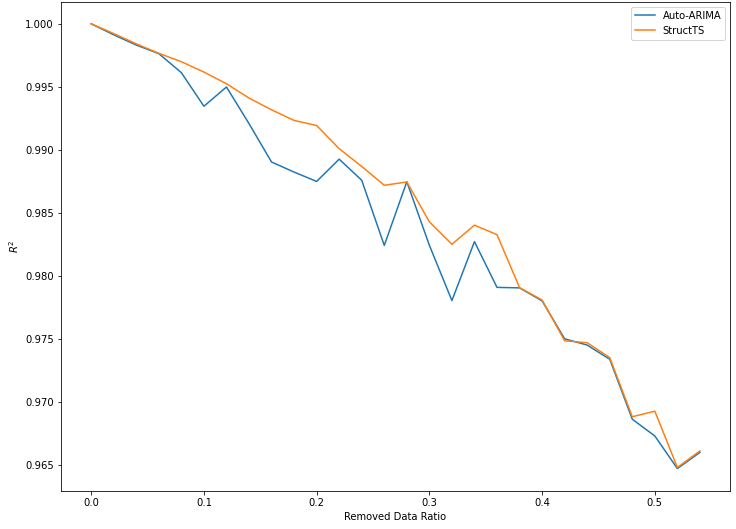
\includegraphics[width=\textwidth]{imp_traffic}
		\caption{Radio traffic load imputation}
		\label{fig:imp_radio_traffic}
	\end{subfigure}%
	\hfill
	\begin{subfigure}{.47\textwidth}
		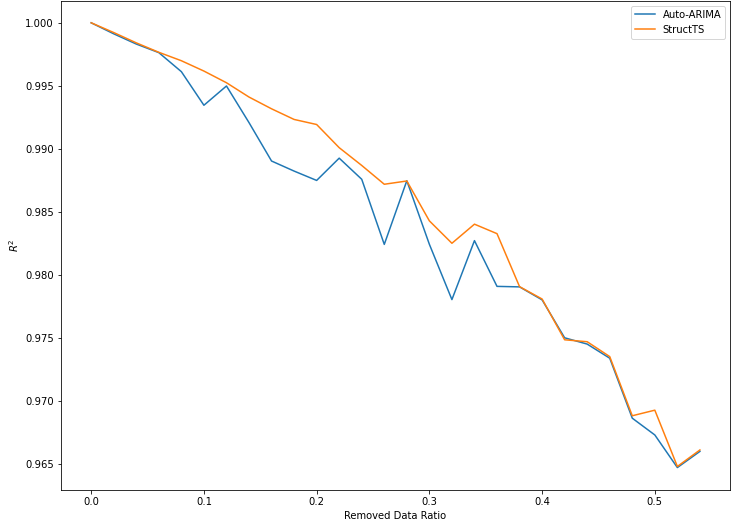
\includegraphics[width=\textwidth]{imp_temp}
		\caption{Cabinet temperature}
		\label{fig:imp_temp}
	\end{subfigure}
	\caption{Imputation experiments good results}
	\label{fig:imp_exp_good}
\end{figure}

Although the plots above show promising results, there are other cases where the experiment did not perform as expected. 

\pagebreak

\subsubsection*{Unintuitive $R^2$ values}

There are cases in which Auto-ARIMA estimation show poor and even negative $R^2$ values as shown in Figure \ref{fig:imp_exp_issue}. The latter are unintuitive results, as $R^2$ values are expected to be limited to the $[0,1]$ interval. 

Nonetheless, this is meant only for linear models, where the worst fitted model is assumed to be the observations mean[add citation]. Thus, having negative $R^2$ values implies that the observations mean explains more variance than the fitted model.

\begin{figure}[hptb]
	\begin{subfigure}{.47\textwidth}
		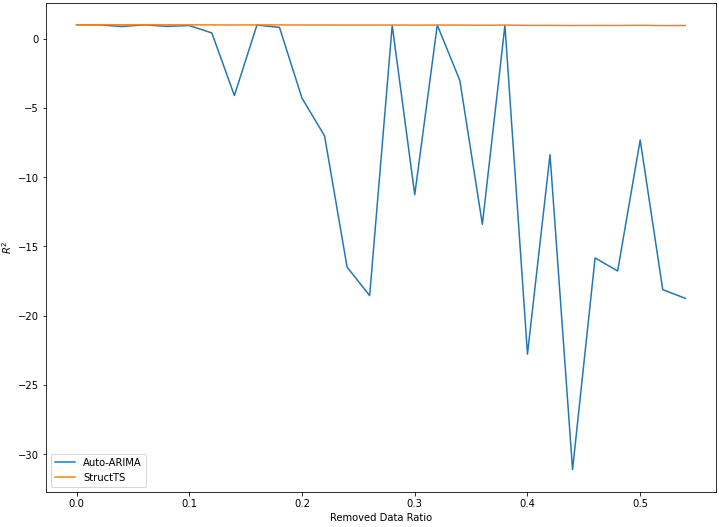
\includegraphics[width=\textwidth]{imp_sys_voltage}
		\caption{\ac{pdu} system voltage imputation}
		\label{fig:imp_pdu_sys_voltage}
	\end{subfigure}%
	\hfill
	\begin{subfigure}{.47\textwidth}
		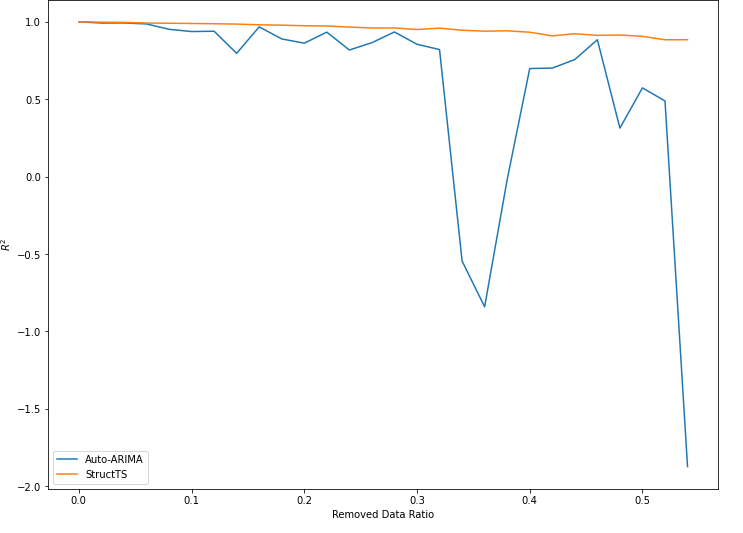
\includegraphics[width=\textwidth]{imp_power_load}
		\caption{Average \ac{psu} utilization imputation}
		\label{fig:imp_psu_load}
	\end{subfigure}
	\caption{Imputation experiments good results}
	\label{fig:imp_exp_issue}
\end{figure}

\subsubsection*{Optim convergence failures}

The model estimation threw runtime exceptions for some features due to the R code calls to the \texttt{optim} library not converging. These exceptions were found to be an actual bug in the library that occurs when the function being optimised tends to a constant value. 

A dedicated routine was written to catch whenever this exception was thrown and run a simple interpolation instead of estimating the model.

\begin{figure}[H]
	\centering
	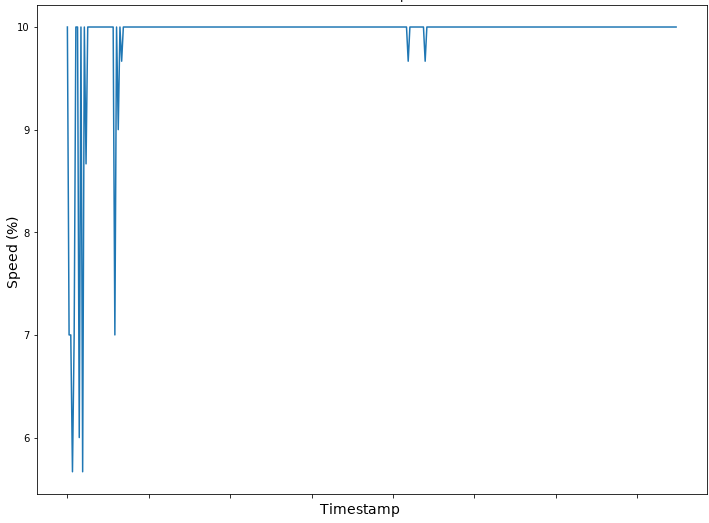
\includegraphics[width=0.55\linewidth]{imp_conv_issue}
	\caption{Problematic signals for imputeTS}
	\label{fig:imp_conv_issue}
\end{figure}

\section{Database construction algorithm}

It has been implemented a pipeline to build a unified and non-corrupted database from the sparsed raw files so that the forecasting section could learn from reliable data.

In the Figure, it is shown how the implemented blocks interact with each other to accomplish this task.

\begin{figure}[H]
	\centering
	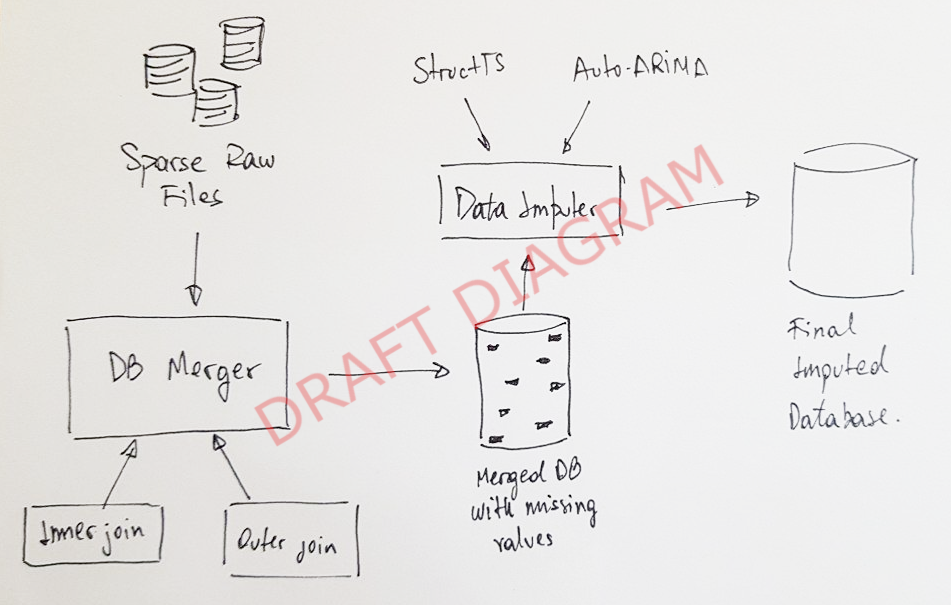
\includegraphics[width=0.65\linewidth]{db_construction_algorithm}
	\caption{Database construction algorithm}
	\label{fig:db_construction_algorithm}
\end{figure}

